\chapter{Uživatelská příručka}
\label{chap:userGuide}
\section{Požadavky}
Vyžaduje verzi OpenGL 3 nebo vyšší, navíc je potřeba balíček Microsoft Visual C++ 2015 Redistributable, který je ve formě .dll přibalen. Pokud by s ním přesto byly problémy, tak doporučuji stáhnout  a nainstalovat jeho aktuální verzi z \url{https://www.microsoft.com/cs-CZ/download/details.aspx?id=53840}
\section{Základní ovladání}
Při spuštění se program otevře v výchozím grafickém režimu, kde dojde k nahrání zabudované Sluneční soustavy. Simulace se ovládá pomocí grafického rozhraní - Obrázek \ref{fig:GUI1}.\\
\begin{figure}
	\caption{Grafické rozhraní programu}
	\label{fig:GUI1} 
	\centering
	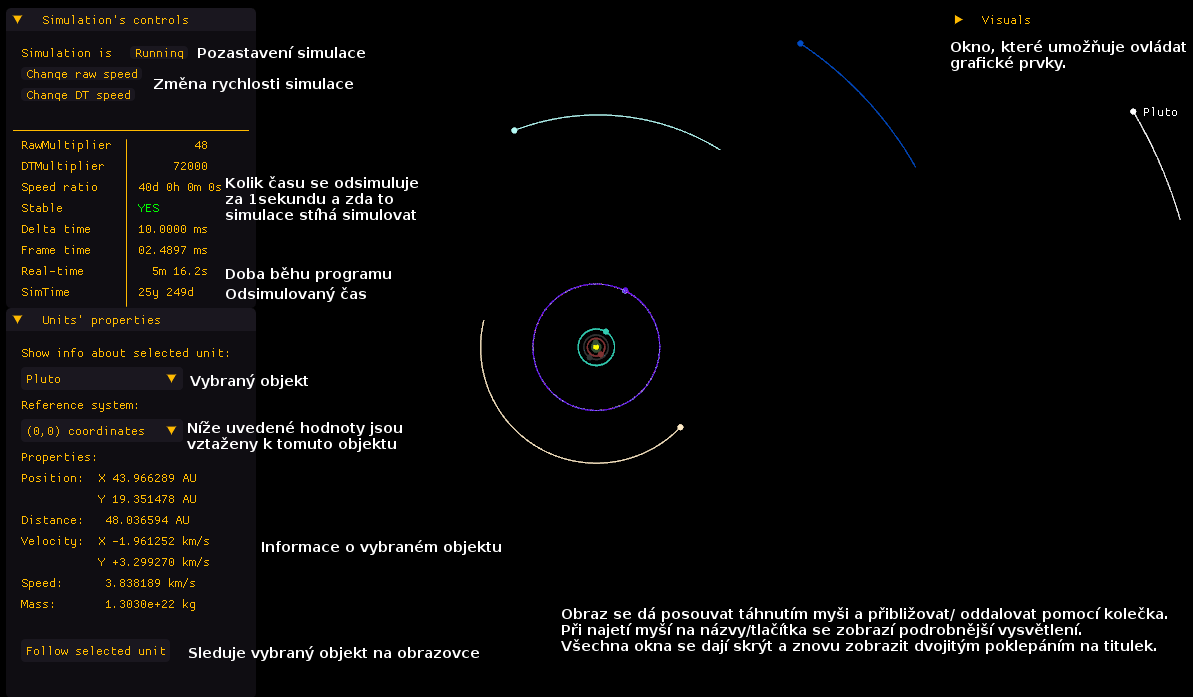
\includegraphics[scale=0.5]{Figs/GUI1_edited}
\end{figure}
\FloatBarrier
\section{Pokročilé možnosti}
Program také nabízí pokročilejší ovládání pomocí příkazové řádky, s níž je možné načítat simulovaná data ze souboru, vybrat si integrační metody a také možnost zaznamenat a následně přehrát uložené simulace.
Pro vypsání nápovědy a všech dostupných příkazů v českém jazyce použijte:
\ \texttt{\textbf{SolarSystem.exe -help -cz}}

Uveďme zde alespoň pár dalších příkladů různých příkazů:
\begin{enumerate}
	\item \texttt{\textbf{SolarSystem.exe vstup.txt}} \\
	Načte vstupní data z formátovaného souboru \texttt{vstup.txt} a spustí simulaci, která bude běžet v reálném čase a zobrazovat se v okně 1200x700 s uživatelským rozhraním.
	\item \texttt{\textbf{SolarSystem.exe -sim -p formatted -i vstup.txt -m RK4 -v win}} \\
	 Ekvivalentní zápis předchozího příkladu. S explicitním použitím modulů.
	\item \texttt{\textbf{SolarSystem.exe -sim -rm 24 -dm 3600 -x 300}} \\
	Spustí podobnou simulaci jako v 1. příkladu. Akorát bude mít 3600x větší integrační krok a bude probíhat 10x rychleji. Ve výsledku se tedy odsimuluje jeden den za jednu reálnou sekundu. Simulace se vypne po 5 minutách běhu.
	\item \texttt{\textbf{SolarSystem.exe -record -r zaznam.replay -p formatted -i vstup.txt -o vystup.txt -m semiEuler -rm 24 -dm 3600 -x 60}}\\
	Zaznamená 60 sekundovou simulaci do souboru \texttt{zaznam.replay}, vstupní data načte z formátovaného souboru \texttt{vstup.txt} a výsledná data uloží do \texttt{vystup.txt} ve stejném formátu. Simulace bude simulovat jeden den za jednu sekundu pomocí semi-implicitní Eulerovy integrační metody. Simulace se spustí v grafickém prostředí stejně jako v 1. příkladě.
	\item  \texttt{\textbf{SolarSystem.exe zaznam.replay}}\\
	Přehraje zaznamenanou simulaci z předchozího příkladu v grafickém prostředí.
\end{enumerate}
K .exe souboru je přiložen vzorový formátovaný text \texttt{vstup.txt} a také jeden záznam simulace \texttt{zaznam.replay}.
Přesný popis formátovaného vstupního souboru je uveden v sekci \ref{sec:strukturaDat} . Pro detailní vysvětlení parametrů simulace je k dispozici popis v sekci \ref{sec:startMetoda}.


\chapter{Kompilace programu}
\section{Git}
Tato dokumentace spolu se zdrojovými kódy programu je veřejně dostupná na:
\begin{center}
\texttt{https://bitbucket.org/Quimby/solar/src}
\end{center}
Popřípadě přímo stažitelná pomocí git HTTPS\eqref{git:https} nebo SSH\eqref{git:ssh}:
\begin{align}
	\label{git:https}
	\texttt{https://Quimby@bitbucket.org/Quimby/solar.git}\\
	\label{git:ssh}
	\texttt{git@bitbucket.org:Quimby/solar.git}
\end{align}
\section{Windows}
Program byl tvořen v programu Visual Studio 2015 Community Edition, takže je zde už předpřipravený .sln projekt, který by měl obsahovat vše potřebné pro správné zkompilování.
\section{Linux}
Program by zde měl být teoreticky také plně funkční, avšak není zde zatím žádný pomocný projekt ani makefile. Kdyžtak je potřeba nejdříve stáhnout a zkompilovat externí knihovny - GLFW, GLEW. Návod by měl být na jejich oficiálních stránkách . Momentálně obě knihovny nabízí vytvoření potřebných souborů pomocí programu CMake, takže kompilace by neměla být těžká. Dále kompilace samotného programu vyžaduje minimálně flag \texttt{GLEW\_STATIC} a také include path do složky obsahující složku \texttt{Source/}(defaultně se nachází ve složce SolarSystem) a samozřejmě slinkovat obě knihovny, ale pak by už mělo vše fungovat. 